\chapter{信号通过线性系统}%
\label{cha:信号通过线性系统}

\section{实验目的}%
\label{sec:实验目的\arabic{chapter}}

\begin{enumerate}
	\item 观察对称方波通过线性系统后波形的失真,了解线性系统频率特性对信号传输的影响;
	\item 测试线性系统的时域特性——阶跃响应。
\end{enumerate}

\section{实验原理及方法}%
\label{sec:实验原理及方法\arabic{chapter}}

本实验所采用的激励信号为对称方波,此信号具有极丰富的频率分量,当这样的信号通过线性系统时,若系统的频率响应特性不满足无失真传输的条件,那么方波中的某些频率分量必然被抑制,造成输出信号与输入信号的不同(失真);若系统的频率响应特性不同则被抑制的频率亦会不同,输出信号的形状也不相同。

\begin{enumerate}
	\item 对称方波通过微分电路(高通滤波器)

		微分电路如图\ref{fig:微分电路}所示,该电路的时间常数为$ T=RC $,若输入的方波的脉宽$ \tau $远大于电路的时间常数$ T $,则输出的波形为尖脉冲;若方波的脉宽$ \tau $远小于电路的时间常数$ T $,则输出的波形近似方波如图\ref{fig:微分电路}所示。

		\begin{figure}[htpb]
			\centering
			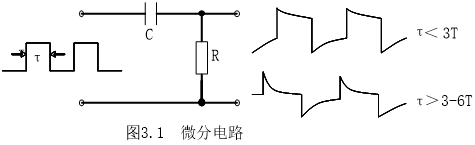
\includegraphics[width=0.8\linewidth]{3-2.png}
			\caption{微分电路}
			\label{fig:微分电路}
		\end{figure}

		从频域角度分析,微分电路实质上是一个高通滤波器,其系统函数为:$ H(s)= \dfrac{s}{s+ \dfrac{1}{RC} } $,其截止频率为:$ \Omega_\text{c}= \dfrac{1}{RC} $。

		当方波通过高通滤波器时,基波及低次谐波分量将受到衰减,从而产生平顶失真;而且$ RC $越小(截止频率越大)失真越大,即波形越尖;反之波形失真较小,波形较平坦。
	\item 对称方波通过积分电路(低通滤波器)

		积分电路如图\ref{fig:积分电路}所示,该电路的时间常数为$ T=RC $,若输入的方波的脉宽$ \tau $远大于电路的时间常数$ T $,则输出的波形近似方波;若方波的脉宽$ \tau $远小于电路的时间常数$ T $,则输出的精度大大降低,波形接近三角波如图\ref{fig:积分电路}所示。

		\begin{figure}[htpb]
			\centering
			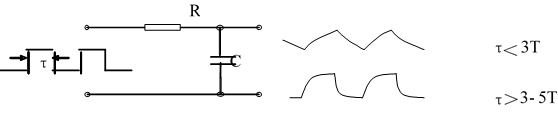
\includegraphics[width=0.8\linewidth]{3-2a.png}
			\caption{积分电路}
			\label{fig:积分电路}
		\end{figure}

		同样从频域角度分析,积分电路实质上是一个低通滤波器,其系统函数为:$ H(s)= \dfrac{1}{RC} \dfrac{1}{s+ \dfrac{1}{RC} } $,其截止频率为:$ \Omega_\text{c}= \dfrac{1}{RC} $。

		当方波通过低通滤波器时,高次谐波分量将受到衰减,因而输出信号中只有低频分量,因此输出波形的前沿变倾斜;而且$ RC $越大(截止频率越小),前沿倾斜越大,即波形失真越大;反之波形失真较小,波形较接近方波。
	\item 对称方波通过LC低通滤波器

		LC低通滤波器的电路如图\ref{fig:LC 低通滤波器}所示。

		\begin{figure}[htpb]
			\centering
			\includegraphics{LC.pdf}
			\caption{LC 低通滤波器}
			\label{fig:LC 低通滤波器}
		\end{figure}

		LC低通滤波器的截止频率为:$ \Omega_\text{c}=\dfrac{2}{\sqrt{(L_1+L_2)C}} $

		当对称矩形脉冲(方波)通过低通滤波器时,频率高于$ f_\text{c} $的谐波分量将被截止(或衰减)到达不了输出端,只有$ f<f_\text{c}  $的低频分量可以到达输出端,所以当不同频率的方波通过此滤波器时,能通过的频率分量将不同;方波的频率越高,通过的频率分量越少即失真越大。

		\begin{enumerate}
			\item 若方波的基波分量$ f_1<f_\text{c} $,而三次谐波分量$ f_3<f_\text{c} $;则能通过的只有$ f_1 $,即输出端为正弦信号;
			\item 若方波的三次谐波分量$ f_3<f_\text{c} $,而五次谐波分量$ f_5<f_\text{c} $,则能通过的只有$ f_1 $,$ f_3 $,即输出端信号为基次和三次谐波的合成波形;
			\item 若方波的频率$ f<<f_\text{c} $,则通过的谐波分量大大增加输出波形更接近方波但此时在波形的前沿将出现一峰值这就是吉伯斯现象。
		\end{enumerate}
	\item 阶跃响应的观测

		阶跃响应则是指单位阶跃信号作用下系统的零状态响应。我们用冲激响应和阶跃响应来描述系统的时域特性。由于普通示波器无法捕捉到$ t=0 $时刻的瞬间跳变,所以我们用方波作为激励信号;只要方波的重复周期$ T_1 $足够大 ($ T_1>> $阶跃响应建立的时间$ t_r $) ,则方波前半周的信号就可以看成是阶跃信号,若将此方波通过系统其响应的前半周就可以认为是阶跃响应。本实验的线性系统为一串联谐振系统,如图\ref{fig:串联谐振电路}所示。

		\begin{figure}[htpb]
			\centering
			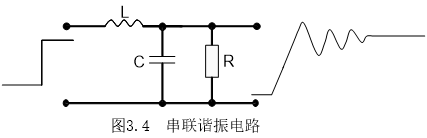
\includegraphics[width=0.8\linewidth]{3-2c.png}
			\caption{串联谐振电路}
			\label{fig:串联谐振电路}
		\end{figure}

		当方波加至串联谐振电路时,将引起电路的谐振,振荡的频率为$ \Omega_0=\dfrac{1}{\sqrt{LC}} $,此时只要满足方波的频率$ \Omega_1<<\Omega_0 $,就可以把响应的前半周认为是阶跃响应。
\end{enumerate}

\section{实验前预习内容}%
\label{sec:实验前预习内容\arabic{chapter}}

\begin{Exercise}
	计算微分电路的截止频率($ R=\SI{10}{k\ohm},C=\SI{1000}{pF} $),并画出幅频特性曲线。
\end{Exercise}

\begin{Answer}
	截止频率见图\ref{fig:运行界面code33.m},幅频特性曲线见图\subref{fig:微分电路幅频特性曲线}。
\end{Answer}

\begin{Exercise}
	计算积分电路的截止频率($ R=\SI{20}{k\ohm},C=\SI{1000}{pF} $),并画出幅频特性曲线。
\end{Exercise}

\begin{Answer}
	截止频率见图\ref{fig:运行界面code33.m},幅频特性曲线见图\subref{fig:积分电路幅频特性曲线}。
\end{Answer}

\begin{Exercise}
	计算LC低通滤波器的截止频率($ L=\SI{10}{mH},C=\SI{0.1}{\micro F} $)。
\end{Exercise}

\begin{Answer}
	截止频率见图\ref{fig:运行界面code33.m}。
\end{Answer}

\langCVfile[Matlab][code:code33.m][Matlab]{code33.m}{src/code33.m}

\begin{figure}[htpb]
	\centering
	\matlablightfile{MATLAB Command Window}{src/code33.txt}
	\caption{运行界面}
	\label{fig:运行界面code33.m}
\end{figure}

\begin{figure}[htpb]
	\centering
	\begin{subfigure}[htpb]{.45\linewidth}
		\centering
		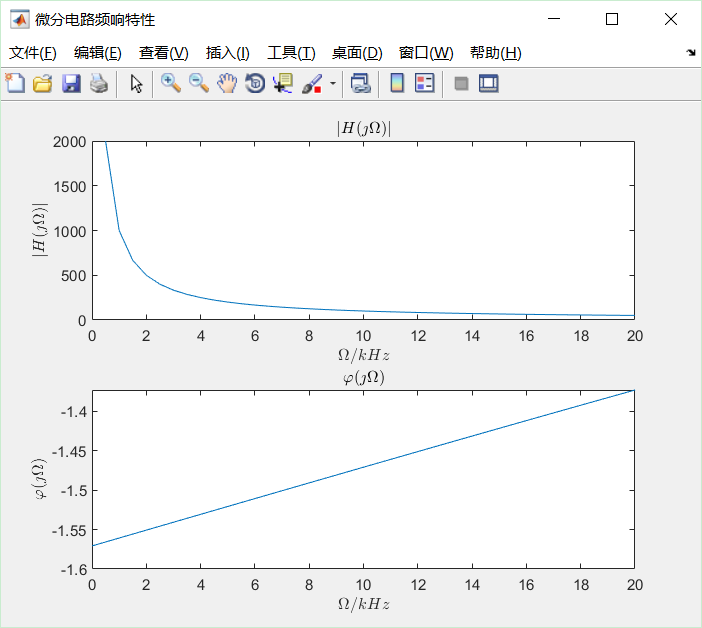
\includegraphics[width=\linewidth]{D.png}
		\caption{微分电路幅频特性曲线}
		\label{fig:微分电路幅频特性曲线}
	\end{subfigure}
	\quad
	\begin{subfigure}[htpb]{.45\linewidth}
		\centering
		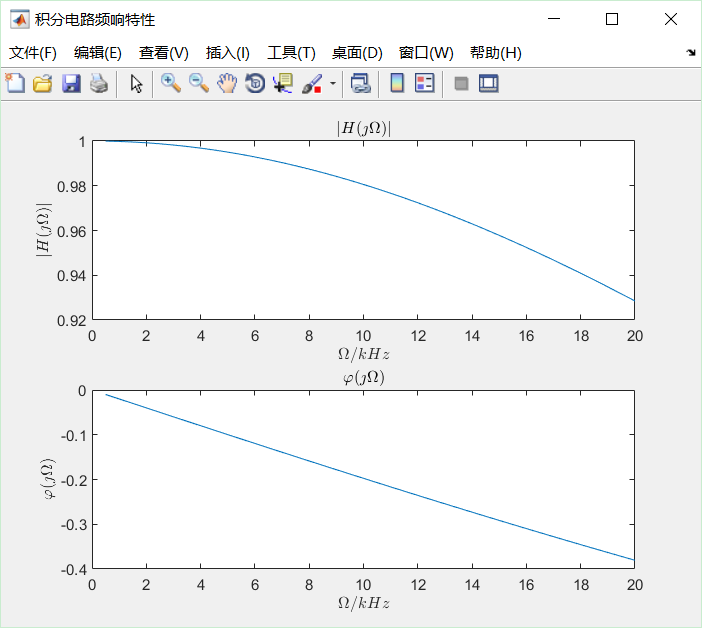
\includegraphics[width=\linewidth]{S.png}
		\caption{积分电路幅频特性曲线}
		\label{fig:积分电路幅频特性曲线}
	\end{subfigure}
	\caption{电路幅频特性曲线}
	\label{fig:电路幅频特性曲线}
\end{figure}

\begin{Exercise}
	用Matlab画出图\ref{fig:串联谐振电路}所示串联谐振电路的阶跃响应图形。
\end{Exercise}

\begin{Answer}
	阶跃响应波形见图\ref{fig:阶跃响应}。
\end{Answer}

\langCVfile[Matlab][code:code334.m][Matlab]{code334.m}{src/code334.m}

\begin{figure}[htpb]
	\centering
	\matlablightfile{MATLAB Command Window}{src/code334.txt}
	\caption{运行界面}
	\label{fig:运行界面code334.m}
\end{figure}

\begin{figure}[htpb]
	\centering
	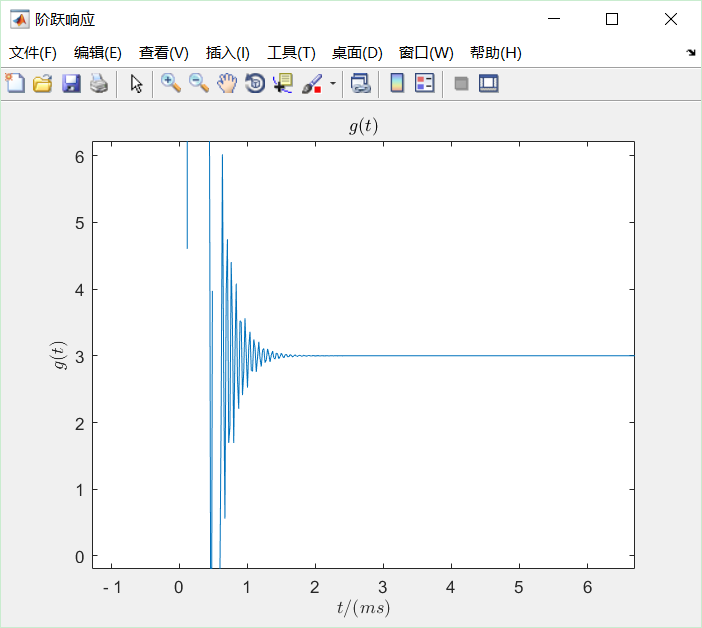
\includegraphics[width=0.6\linewidth]{stepResponse.png}
	\caption{阶跃响应}
	\label{fig:阶跃响应}
\end{figure}

\newpage

\section{实验原理图}%
\label{sec:实验原理图\arabic{chapter}}

\begin{figure}[htpb]
	\centering
	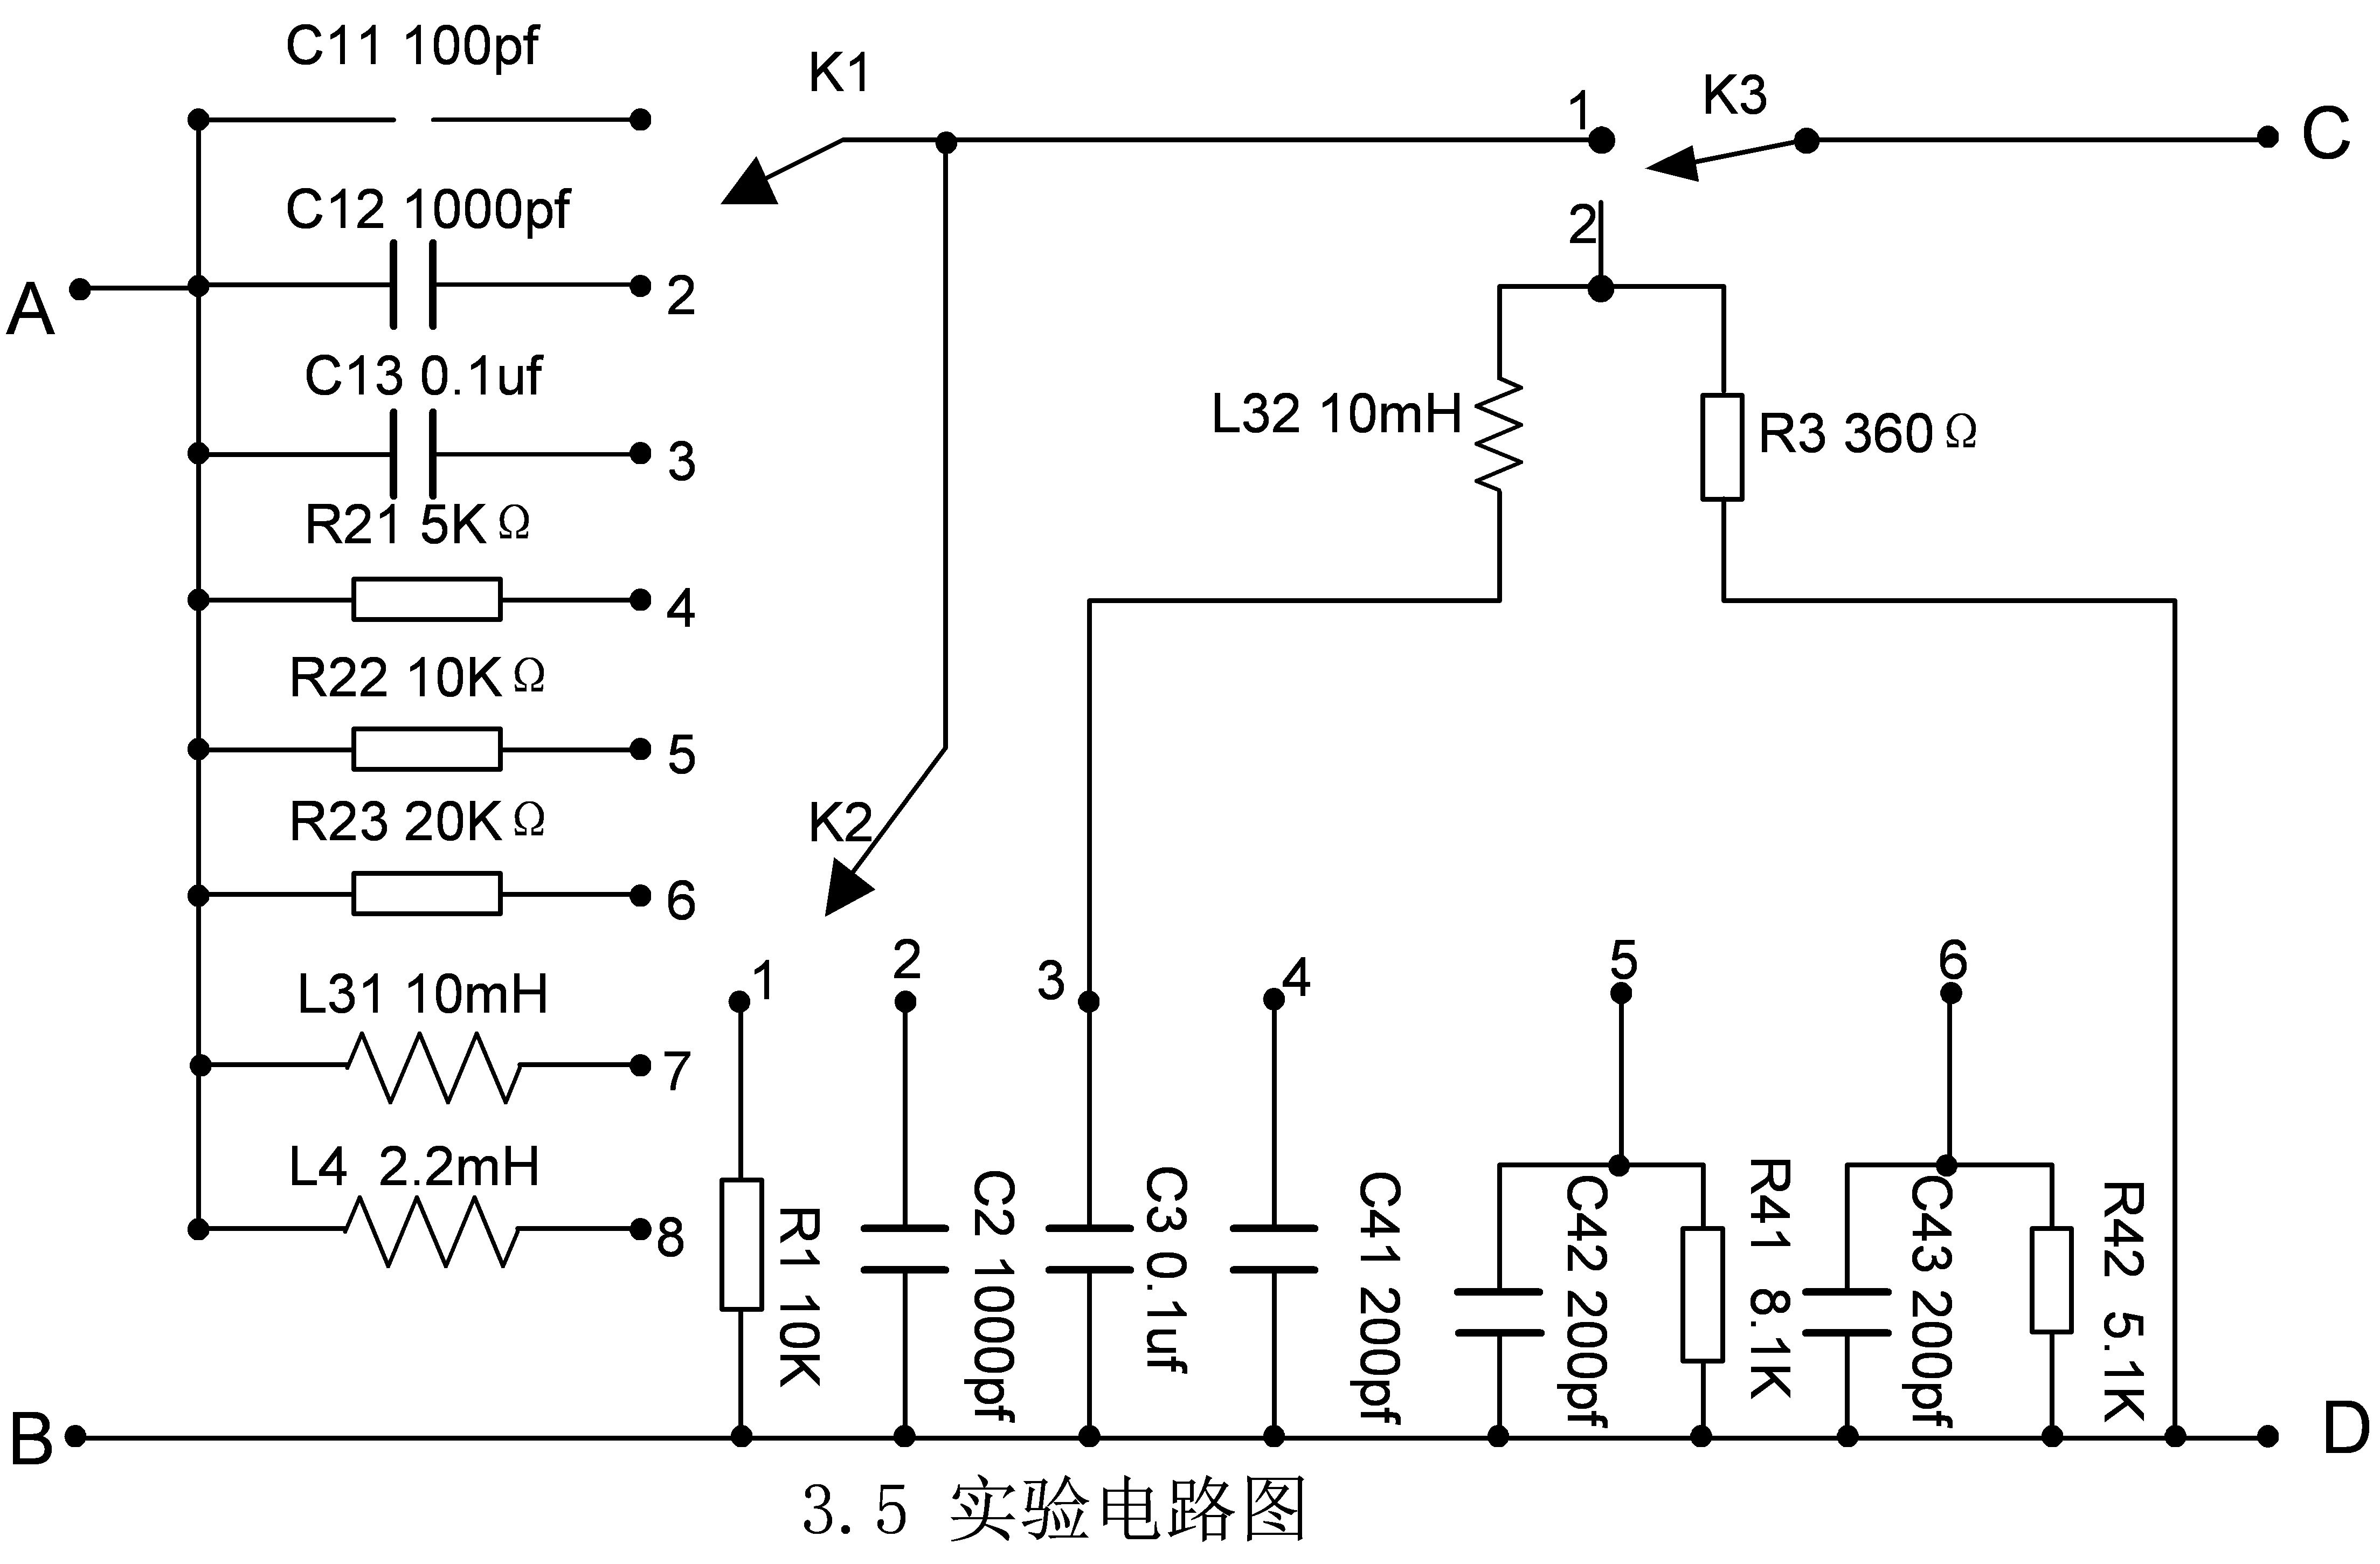
\includegraphics[width=0.6\linewidth]{3-4.png}
	\caption{实验原理图\arabic{chapter}}
	\label{fig:实验原理图\arabic{chapter}}
\end{figure}

\section{实验内容及步骤}%
\label{sec:实验内容及步骤\arabic{chapter}}

将函数发生器的输出CH1输出波形调为方波,频率调为\SI{10}{kHz},幅度调为$ V_\text{pp}=\SI{5}{V} $,并将此方波接实验板的A、B两点,示波器接实验板上的输出端CD两点。

\subsection{将电路接成微分电路,观察并记录波形}%
\label{sub:将电路接成微分电路,观察并记录波形}

将实验电路中的K2置于1,K3置于1, K1分别置于1,2,3,观察并记录波形;计算时间常数$ T=RC $的值,并与方波的脉宽$ \tau $进行比较说明时间常数T的变化对输出波形的影响。并从频域的角度(系统的频率特性)分析输出波形产生平顶失真的原因。

\begin{figure}[htpb]
	\centering
	\begin{subfigure}[htpb]{.31\linewidth}
		\centering
		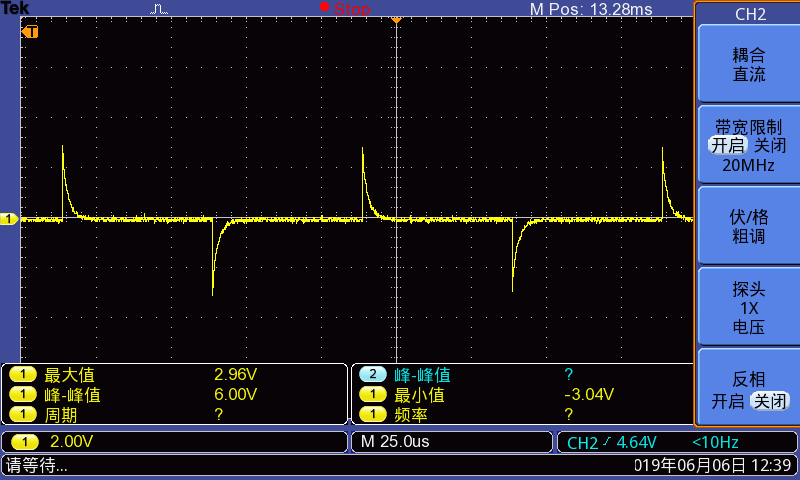
\includegraphics[width=\linewidth]{TEK311.png}
		\caption{微分电路波形图\arabic{subfigure}}
		\label{fig:微分电路波形图\arabic{subfigure}}
	\end{subfigure}
	\quad
	\begin{subfigure}[htpb]{.31\linewidth}
		\centering
		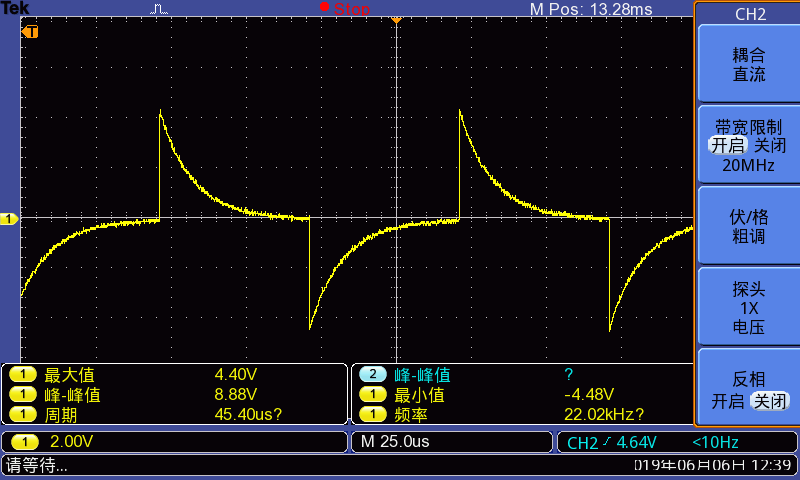
\includegraphics[width=\linewidth]{TEK312.png}
		\caption{微分电路波形图\arabic{subfigure}}
		\label{fig:微分电路波形图\arabic{subfigure}}
	\end{subfigure}
	\quad
	\begin{subfigure}[htpb]{.31\linewidth}
		\centering
		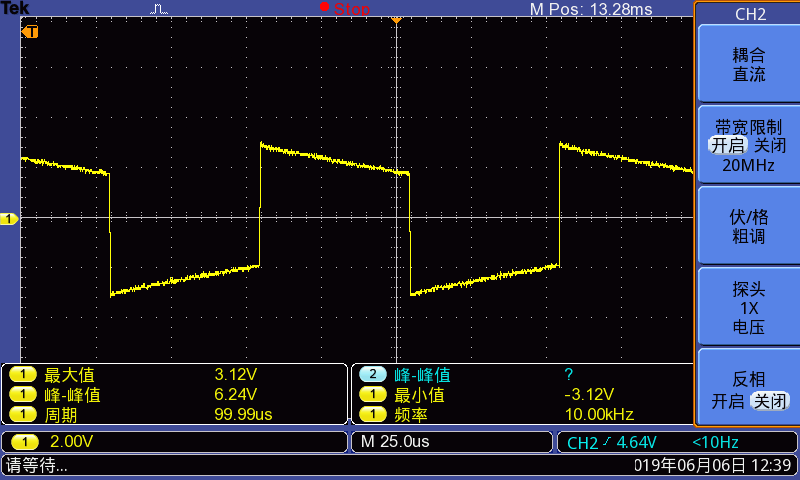
\includegraphics[width=\linewidth]{TEK313.png}
		\caption{微分电路波形图\arabic{subfigure}}
		\label{fig:微分电路波形图\arabic{subfigure}}
	\end{subfigure}
	\caption{微分电路波形图}
	\label{fig:微分电路波形图}
\end{figure}

\subsection{将电路接成积分电路,观察并记录波形}%
\label{sub:将电路接成积分电路,观察并记录波形}

将实验电路中的K2置于2,K3置于1, K1分别置于4,5,6,观察并记录波形;计算时间常数$ T=RC $的值,并与方波的脉宽$ \tau $进行比较,说明时间常数T的变化对输出波形的影响。并从频域的角度(系统的频率特性)分析输出波形产生平顶失真的原因。

\begin{figure}[htpb]
	\centering
	\begin{subfigure}[htpb]{.31\linewidth}
		\centering
		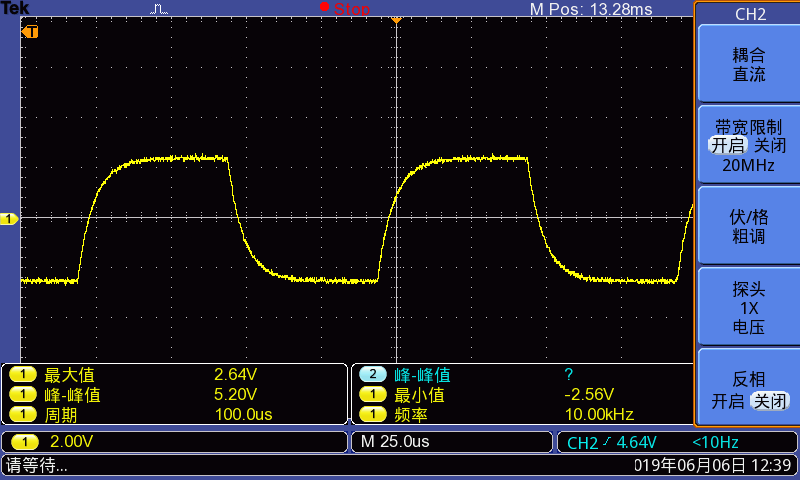
\includegraphics[width=\linewidth]{TEK321.png}
		\caption{积分电路波形图\arabic{subfigure}}
		\label{fig:积分电路波形图\arabic{subfigure}}
	\end{subfigure}
	\quad
	\begin{subfigure}[htpb]{.31\linewidth}
		\centering
		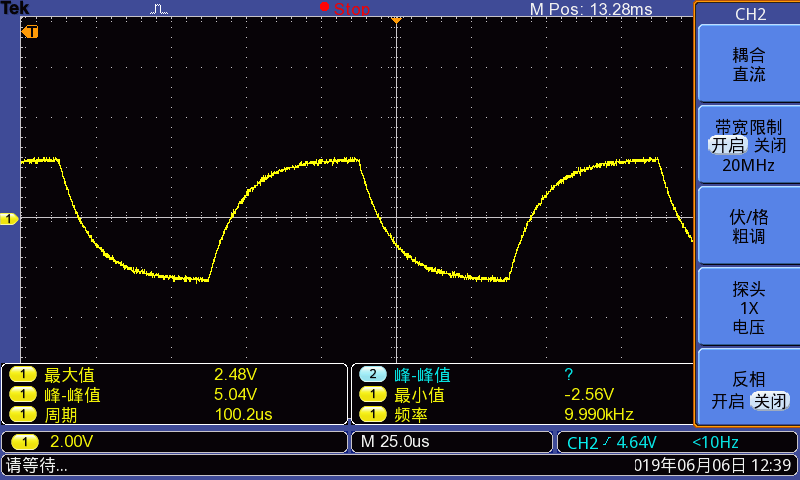
\includegraphics[width=\linewidth]{TEK322.png}
		\caption{积分电路波形图\arabic{subfigure}}
		\label{fig:积分电路波形图\arabic{subfigure}}
	\end{subfigure}
	\quad
	\begin{subfigure}[htpb]{.31\linewidth}
		\centering
		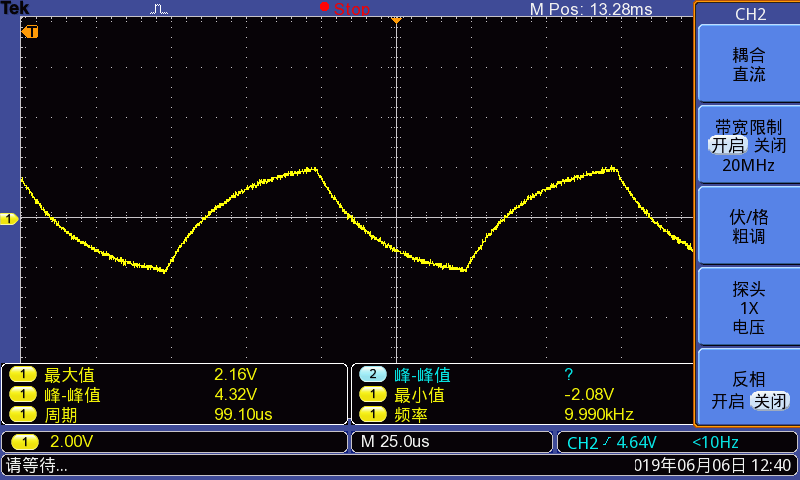
\includegraphics[width=\linewidth]{TEK323.png}
		\caption{积分电路波形图\arabic{subfigure}}
		\label{fig:积分电路波形图\arabic{subfigure}}
	\end{subfigure}
	\caption{积分电路波形图}
	\label{fig:积分电路波形图}
\end{figure}

\subsection{将电路接成LC低通滤波器,观察并记录波形}%
\label{sub:将电路接成LC低通滤波器,观察并记录波形}

将实验电路中的K1置于7,K2置于3, K3置于2,观察并记录波形;然后改变信号源的频率 使之分别满足下面三个条件:\ding{172}$ f<f_\text{c}<3f $,\ding{173}$ 3f<f_\text{c}<5f $,\ding{174}$ f<<f_\text{c}(f_\text{c}=\SI{7.1}{kHz})$;分别记录三种情况下的输出波形,并从频域角度进行解释。

\begin{figure}[htpb]
	\centering
	\begin{subfigure}[htpb]{.31\linewidth}
		\centering
		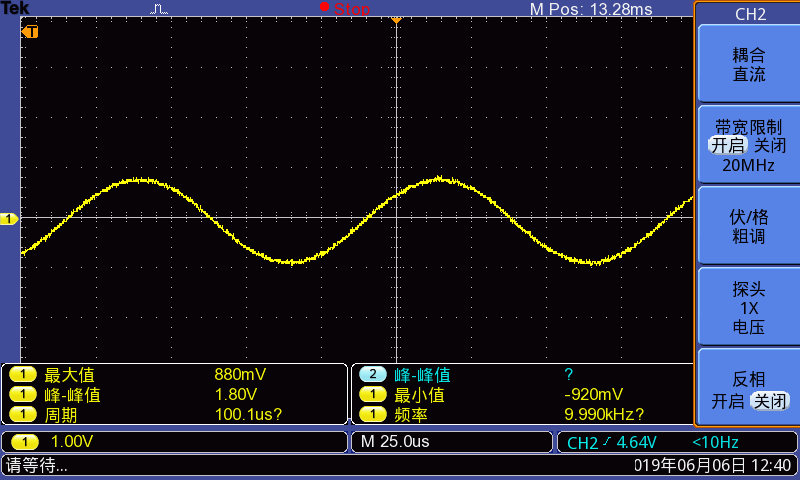
\includegraphics[width=\linewidth]{TEK331.png}
		\caption{LC低通滤波器波形图\arabic{subfigure}}
		\label{fig:LC低通滤波器波形图\arabic{subfigure}}
	\end{subfigure}
	\quad
	\begin{subfigure}[htpb]{.31\linewidth}
		\centering
		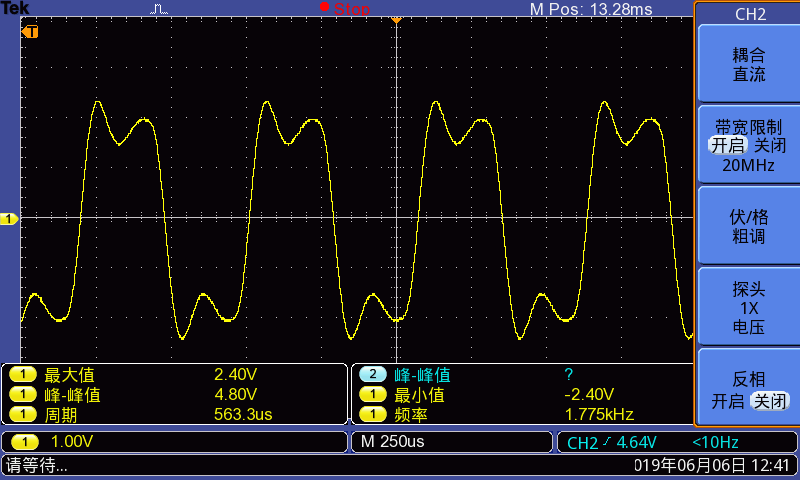
\includegraphics[width=\linewidth]{TEK332.png}
		\caption{LC低通滤波器波形图\arabic{subfigure}}
		\label{fig:LC低通滤波器波形图\arabic{subfigure}}
	\end{subfigure}
	\quad
	\begin{subfigure}[htpb]{.31\linewidth}
		\centering
		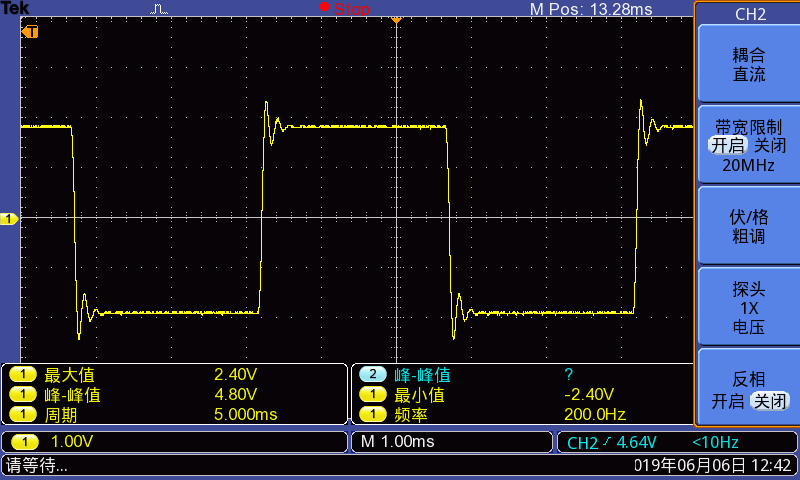
\includegraphics[width=\linewidth]{TEK333.png}
		\caption{LC低通滤波器波形图\arabic{subfigure}}
		\label{fig:LC低通滤波器波形图\arabic{subfigure}}
	\end{subfigure}
	\caption{LC低通滤波器波形图}
	\label{fig:LC低通滤波器波形图}
\end{figure}

\subsection{将电路接成串联谐振回路,观察阶跃响应波形并记录}%
\label{sub:将电路接成串联谐振回路,观察阶跃响应波形并记录}

首先将信号源的频率调回\SI{10}{kHz},K1置于8,K3置于1,K2分别置于4,5,6,观察电路在不同损耗电阻值时的阶跃响应波形并记录。

\begin{figure}[htpb]
	\centering
	\begin{subfigure}[htpb]{.31\linewidth}
		\centering
		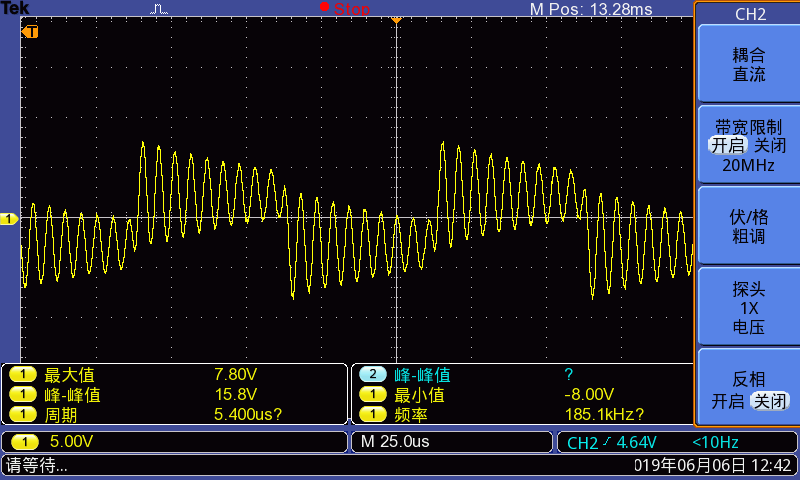
\includegraphics[width=\linewidth]{TEK341.png}
		\caption{串联谐振回路波形图\arabic{subfigure}}
		\label{fig:串联谐振回路波形图\arabic{subfigure}}
	\end{subfigure}
	\quad
	\begin{subfigure}[htpb]{.31\linewidth}
		\centering
		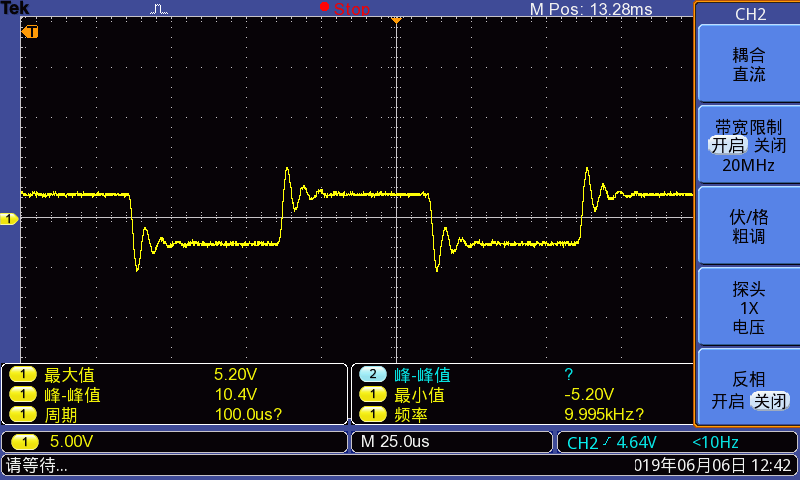
\includegraphics[width=\linewidth]{TEK342.png}
		\caption{串联谐振回路波形图\arabic{subfigure}}
		\label{fig:串联谐振回路波形图\arabic{subfigure}}
	\end{subfigure}
	\quad
	\begin{subfigure}[htpb]{.31\linewidth}
		\centering
		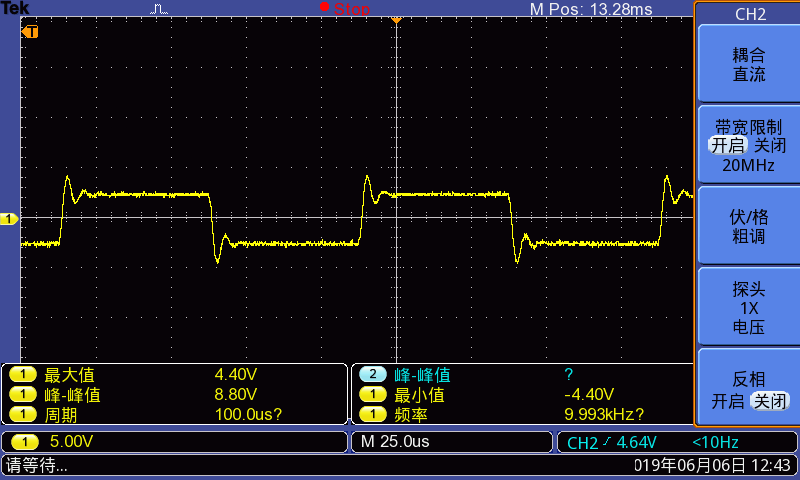
\includegraphics[width=\linewidth]{TEK343.png}
		\caption{串联谐振回路波形图\arabic{subfigure}}
		\label{fig:串联谐振回路波形图\arabic{subfigure}}
	\end{subfigure}
	\caption{串联谐振回路波形图}
	\label{fig:串联谐振回路波形图}
\end{figure}

\section{实验仪器及设备}%
\label{sec:实验仪器及设备\arabic{chapter}}

双踪示波器一台,函数发生器一台,实验板一块。

\section{实验报告要求}%
\label{sec:实验报告要求\arabic{chapter}}

\begin{Exercise}
	叙述实验内容及实验步骤。
\end{Exercise}

\begin{Answer}
	实验内容及实验步骤见第\ref{sec:实验内容及步骤\arabic{chapter}}节。
\end{Answer}

\begin{Exercise}
	详细画出实验内容\ref{sub:将电路接成微分电路,观察并记录波形}至\ref{sub:将电路接成LC低通滤波器,观察并记录波形}中要求记录得的波形,并对所得波形进行相应的理论解释。
\end{Exercise}

\begin{Answer}
	实验内容\ref{sub:将电路接成微分电路,观察并记录波形}至\ref{sub:将电路接成LC低通滤波器,观察并记录波形}中要求记录得的波形见图\ref{fig:微分电路幅频特性曲线}、\ref{fig:积分电路幅频特性曲线}和\ref{fig:LC低通滤波器波形图}。微分电路是高通滤波,保留了大部分高频分量,高频分量影响变化速率,所以跳变处出现 Gibbs 现象;但丧失了大部低频分量,低频分量携带大部分能量,所以阶跃响应比方波面积减小很多;所以最终出现尖顶失真。积分电路是低通滤波,保留了大部分低频分量,低频分量携带大部分能量,所以阶跃响应比方波面积减小不多,比高频响应更接近方波;但丧失了大部分高频分量,高频分量影响变化速率,所以跳变处没有出现 Gibbs 现象;所以最终出现削顶失真。
\end{Answer}

\begin{Exercise}
	在实验内容\ref{sub:将电路接成串联谐振回路,观察阶跃响应波形并记录}中,比较满足同一条件时信号频率取得较低和相对较高时的两种输出波形。
\end{Exercise}

\begin{Answer}
	信号频率较低时输出波形振荡较平缓。信号频率较高时输出波形振荡较剧烈。
\end{Answer}

\begin{Exercise}
	实验中的LC低通滤波器的过渡带宽如何确定。
\end{Exercise}

\begin{Answer}
	过渡带宽是处于通带和止带之间的数字频率宽度,即$ |w_p-w_s| $。在示波器上测量通带边界点和相邻的止带边界点的距离就是过渡带宽。
\end{Answer}

\begin{Exercise}
	画出实验内容\ref{sub:将电路接成串联谐振回路,观察阶跃响应波形并记录}中观察到的不同损耗时的波形,并说明电路中的电阻$ R $对输出波形有何影响。
\end{Exercise}

\begin{Answer}
	实验内容\ref{sub:将电路接成串联谐振回路,观察阶跃响应波形并记录}中观察到的不同损耗时的波形见图\ref{fig:串联谐振电路}。$ R $越大阶跃响应越接近方波。$ R $越小阶跃响应越接近正弦波。
\end{Answer}

\begin{Exercise}
	将实验内容\ref{sub:将电路接成串联谐振回路,观察阶跃响应波形并记录}中观察到输出波形的前半周与仿真的阶跃响应波形进行比较。
\end{Exercise}

\begin{Answer}
	实验内容\ref{sub:将电路接成串联谐振回路,观察阶跃响应波形并记录}中观察到输出波形见图\ref{fig:串联谐振回路波形图},仿真的阶跃响应波形见图\ref{fig:阶跃响应}。仿真时有意取了接近子图\subref{fig:串联谐振回路波形图2}的$ R, L, C $的值。
\end{Answer}

